% GNUPLOT: LaTeX picture with Postscript
\begingroup
  \makeatletter
  \providecommand\color[2][]{%
    \GenericError{(gnuplot) \space\space\space\@spaces}{%
      Package color not loaded in conjunction with
      terminal option `colourtext'%
    }{See the gnuplot documentation for explanation.%
    }{Either use 'blacktext' in gnuplot or load the package
      color.sty in LaTeX.}%
    \renewcommand\color[2][]{}%
  }%
  \providecommand\includegraphics[2][]{%
    \GenericError{(gnuplot) \space\space\space\@spaces}{%
      Package graphicx or graphics not loaded%
    }{See the gnuplot documentation for explanation.%
    }{The gnuplot epslatex terminal needs graphicx.sty or graphics.sty.}%
    \renewcommand\includegraphics[2][]{}%
  }%
  \providecommand\rotatebox[2]{#2}%
  \@ifundefined{ifGPcolor}{%
    \newif\ifGPcolor
    \GPcolorfalse
  }{}%
  \@ifundefined{ifGPblacktext}{%
    \newif\ifGPblacktext
    \GPblacktexttrue
  }{}%
  % define a \g@addto@macro without @ in the name:
  \let\gplgaddtomacro\g@addto@macro
  % define empty templates for all commands taking text:
  \gdef\gplbacktext{}%
  \gdef\gplfronttext{}%
  \makeatother
  \ifGPblacktext
    % no textcolor at all
    \def\colorrgb#1{}%
    \def\colorgray#1{}%
  \else
    % gray or color?
    \ifGPcolor
      \def\colorrgb#1{\color[rgb]{#1}}%
      \def\colorgray#1{\color[gray]{#1}}%
      \expandafter\def\csname LTw\endcsname{\color{white}}%
      \expandafter\def\csname LTb\endcsname{\color{black}}%
      \expandafter\def\csname LTa\endcsname{\color{black}}%
      \expandafter\def\csname LT0\endcsname{\color[rgb]{1,0,0}}%
      \expandafter\def\csname LT1\endcsname{\color[rgb]{0,1,0}}%
      \expandafter\def\csname LT2\endcsname{\color[rgb]{0,0,1}}%
      \expandafter\def\csname LT3\endcsname{\color[rgb]{1,0,1}}%
      \expandafter\def\csname LT4\endcsname{\color[rgb]{0,1,1}}%
      \expandafter\def\csname LT5\endcsname{\color[rgb]{1,1,0}}%
      \expandafter\def\csname LT6\endcsname{\color[rgb]{0,0,0}}%
      \expandafter\def\csname LT7\endcsname{\color[rgb]{1,0.3,0}}%
      \expandafter\def\csname LT8\endcsname{\color[rgb]{0.5,0.5,0.5}}%
    \else
      % gray
      \def\colorrgb#1{\color{black}}%
      \def\colorgray#1{\color[gray]{#1}}%
      \expandafter\def\csname LTw\endcsname{\color{white}}%
      \expandafter\def\csname LTb\endcsname{\color{black}}%
      \expandafter\def\csname LTa\endcsname{\color{black}}%
      \expandafter\def\csname LT0\endcsname{\color{black}}%
      \expandafter\def\csname LT1\endcsname{\color{black}}%
      \expandafter\def\csname LT2\endcsname{\color{black}}%
      \expandafter\def\csname LT3\endcsname{\color{black}}%
      \expandafter\def\csname LT4\endcsname{\color{black}}%
      \expandafter\def\csname LT5\endcsname{\color{black}}%
      \expandafter\def\csname LT6\endcsname{\color{black}}%
      \expandafter\def\csname LT7\endcsname{\color{black}}%
      \expandafter\def\csname LT8\endcsname{\color{black}}%
    \fi
  \fi
  \setlength{\unitlength}{0.0500bp}%
  \begin{picture}(7200.00,5040.00)%
    \gplgaddtomacro\gplbacktext{%
      \csname LTb\endcsname%
      \put(946,3224){\makebox(0,0)[r]{\strut{}$-1.5$}}%
      \put(946,3483){\makebox(0,0)[r]{\strut{}$-1$}}%
      \put(946,3741){\makebox(0,0)[r]{\strut{}$-0.5$}}%
      \put(946,4000){\makebox(0,0)[r]{\strut{}$0$}}%
      \put(946,4258){\makebox(0,0)[r]{\strut{}$0.5$}}%
      \put(946,4517){\makebox(0,0)[r]{\strut{}$1$}}%
      \put(946,4775){\makebox(0,0)[r]{\strut{}$1.5$}}%
      \put(1291,3004){\makebox(0,0){\strut{}$-2$}}%
      \put(1716,3004){\makebox(0,0){\strut{}$-1$}}%
      \put(2141,3004){\makebox(0,0){\strut{}$0$}}%
      \put(2566,3004){\makebox(0,0){\strut{}$1$}}%
      \put(2991,3004){\makebox(0,0){\strut{}$2$}}%
      \put(176,3999){\rotatebox{-270}{\makebox(0,0){\strut{}$y$}}}%
      \put(2140,2674){\makebox(0,0){\strut{}$x$}}%
    }%
    \gplgaddtomacro\gplfronttext{%
      \csname LTb\endcsname%
      \put(2216,4602){\makebox(0,0)[r]{\strut{}"gnuEllipse1.txt"}}%
    }%
    \gplgaddtomacro\gplbacktext{%
      \csname LTb\endcsname%
      \put(4546,3224){\makebox(0,0)[r]{\strut{}$-1.5$}}%
      \put(4546,3483){\makebox(0,0)[r]{\strut{}$-1$}}%
      \put(4546,3741){\makebox(0,0)[r]{\strut{}$-0.5$}}%
      \put(4546,4000){\makebox(0,0)[r]{\strut{}$0$}}%
      \put(4546,4258){\makebox(0,0)[r]{\strut{}$0.5$}}%
      \put(4546,4517){\makebox(0,0)[r]{\strut{}$1$}}%
      \put(4546,4775){\makebox(0,0)[r]{\strut{}$1.5$}}%
      \put(4891,3004){\makebox(0,0){\strut{}$-2$}}%
      \put(5316,3004){\makebox(0,0){\strut{}$-1$}}%
      \put(5741,3004){\makebox(0,0){\strut{}$0$}}%
      \put(6166,3004){\makebox(0,0){\strut{}$1$}}%
      \put(6591,3004){\makebox(0,0){\strut{}$2$}}%
      \put(3776,3999){\rotatebox{-270}{\makebox(0,0){\strut{}$y$}}}%
      \put(5740,2674){\makebox(0,0){\strut{}$x$}}%
    }%
    \gplgaddtomacro\gplfronttext{%
      \csname LTb\endcsname%
      \put(5816,4602){\makebox(0,0)[r]{\strut{}"gnuEllipse2.txt"}}%
    }%
    \gplgaddtomacro\gplbacktext{%
      \csname LTb\endcsname%
      \put(946,704){\makebox(0,0)[r]{\strut{}$-1.5$}}%
      \put(946,963){\makebox(0,0)[r]{\strut{}$-1$}}%
      \put(946,1221){\makebox(0,0)[r]{\strut{}$-0.5$}}%
      \put(946,1480){\makebox(0,0)[r]{\strut{}$0$}}%
      \put(946,1739){\makebox(0,0)[r]{\strut{}$0.5$}}%
      \put(946,1997){\makebox(0,0)[r]{\strut{}$1$}}%
      \put(946,2256){\makebox(0,0)[r]{\strut{}$1.5$}}%
      \put(1291,484){\makebox(0,0){\strut{}$-2$}}%
      \put(1716,484){\makebox(0,0){\strut{}$-1$}}%
      \put(2141,484){\makebox(0,0){\strut{}$0$}}%
      \put(2566,484){\makebox(0,0){\strut{}$1$}}%
      \put(2991,484){\makebox(0,0){\strut{}$2$}}%
      \put(176,1480){\rotatebox{-270}{\makebox(0,0){\strut{}$y$}}}%
      \put(2140,154){\makebox(0,0){\strut{}$x$}}%
    }%
    \gplgaddtomacro\gplfronttext{%
      \csname LTb\endcsname%
      \put(2216,2083){\makebox(0,0)[r]{\strut{}"gnuEllipse3.txt"}}%
    }%
    \gplgaddtomacro\gplbacktext{%
      \csname LTb\endcsname%
      \put(4546,704){\makebox(0,0)[r]{\strut{}$-1.5$}}%
      \put(4546,963){\makebox(0,0)[r]{\strut{}$-1$}}%
      \put(4546,1221){\makebox(0,0)[r]{\strut{}$-0.5$}}%
      \put(4546,1480){\makebox(0,0)[r]{\strut{}$0$}}%
      \put(4546,1739){\makebox(0,0)[r]{\strut{}$0.5$}}%
      \put(4546,1997){\makebox(0,0)[r]{\strut{}$1$}}%
      \put(4546,2256){\makebox(0,0)[r]{\strut{}$1.5$}}%
      \put(4891,484){\makebox(0,0){\strut{}$-2$}}%
      \put(5316,484){\makebox(0,0){\strut{}$-1$}}%
      \put(5741,484){\makebox(0,0){\strut{}$0$}}%
      \put(6166,484){\makebox(0,0){\strut{}$1$}}%
      \put(6591,484){\makebox(0,0){\strut{}$2$}}%
      \put(3776,1480){\rotatebox{-270}{\makebox(0,0){\strut{}$y$}}}%
      \put(5740,154){\makebox(0,0){\strut{}$x$}}%
    }%
    \gplgaddtomacro\gplfronttext{%
      \csname LTb\endcsname%
      \put(5816,2083){\makebox(0,0)[r]{\strut{}"gnuEllipse4.txt"}}%
    }%
    \gplbacktext
    \put(0,0){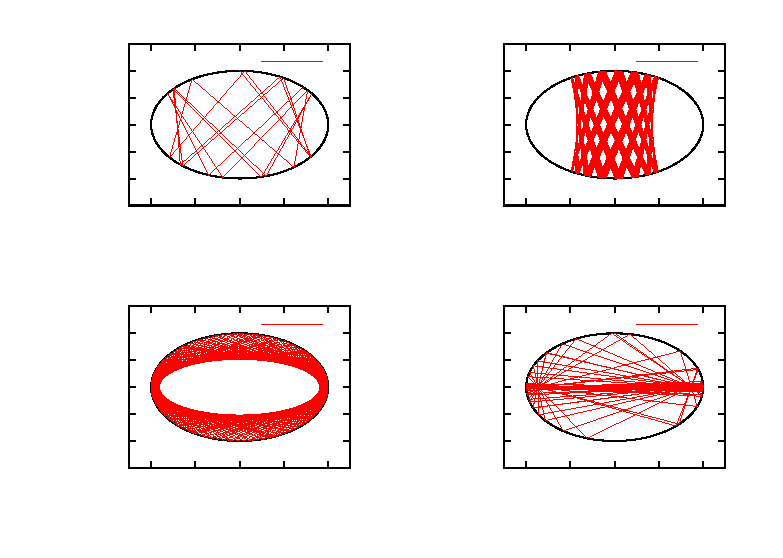
\includegraphics{EllTraj}}%
    \gplfronttext
  \end{picture}%
\endgroup
